\documentclass{standalone}

\usepackage{tikz}
\usepackage{circuitikz}

\tikzset{block/.style = {draw, fill=white, very thick, rectangle, minimum height=1cm, minimum width=2cm},
         lblock/.style={draw,fill=white,very thick, rectangle, minimum height=3cm, minimum width=1cm},
         sum/.style= {draw, fill=white, very thick, circle, node distance=0.5cm}}

         
\begin{document}
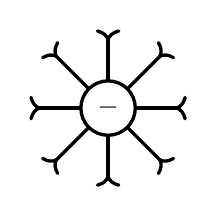
\begin{tikzpicture}[scale=2]
    \draw[>-<, very thick](1.5,0)--(2.5,0);

    \draw[>-<, very thick](2,-0.5)--(2,0.5);


    \draw[>-<, very thick](1.625,-0.375)--(2.375,0.375);
    \draw[>-<, very thick](2.375,-0.375)--(1.625,0.375);

    \node[sum](-)at(2,0){$-$};
\end{tikzpicture}
\end{document}